\chapter{Numerical methods for photonics}
\label{h:numeric}

\begin{quote}
The purpose of computing is insight, not numbers.

--- Richard Hamming
\end{quote}

\begin{quote}
Understanding grows only logarithmically with the number of floating point operations 

--- J.P. Boyd
\end{quote}

\chaptertoc


In this chapter, we will briefly touch upon a number of techniques to numerically solve the wave equation in cases where no analytic solution is available. Four different classes of methods will be introduced.

First, in \textbf{finite difference} methods, we will replace continuous derivatives with discrete approximations on a grid. When applying this to the wave equation in the frequency domain, this results in a linear system, which can be solved in a number of ways. Doing this discretisation in the time domain results in the popular finite-difference time-domain method (FDTD).

The \textbf{finite element} method does not directly solve a differential equation. Rather, it tackles the problem obliquely by converting it into a minimisation procedure. This so-called variational approach has advantages when it comes to e.g. sensitivity to rounding errors.

\textbf{Eigenmode expansion} methods are used in layered photonic structures, in which the fields are expanded in the basis set formed by the eigenmodes of each layer. Thanks to this choice of basis functions that incorporate a lot of the physics of the problem, this approach can be very efficient.

Finally, a more abstract framework is presented, namely the \textbf{method of the weighted residuals}. This framework can be used to generalise a number of individual approaches, like point matching or the Galkerkin method.

Each of these subjects could be the topic of an entire course in its own right, so we will only be able to introduce the basic principle of these methods, without going into any level of detail. What is important however, is to get a feeling for each of these methods, to get to know their strengths and weaknesses, so that you can make the correct choice of tool for any given problem.


\pagebreak

\sectionugent{Finite difference approximation of derivatives}

Let's say we are not interested in the solution to a certain differential equation in the entire domain of interest, but only in a limited number of discrete points inside the simulation domain. The set of discretisation points is called the \textbf{mesh}, and the distance between discretisation points is called the \textbf{mesh size}. A typical choice of 2D mesh is a rectangular one, where you only consider points of the form $(i \Delta x, j \Delta y)$, with $i$ and $j$ integers.

\begin{cue}
What do you think are some advantages and disadvantages of having a small mesh size?  
\end{cue}

Obviously the hope is that as the mesh becomes finer and finer, the solution that we obtain converges more and more to the true solution of the wave equation. However, the price we pay for this consists of increased computational resources (time, memory, ...).

\begin{marginfigure}[-2.0cm]
  % credits: Wikipedia
  % url: https://en.wikipedia.org/wiki/Brook_Taylor
  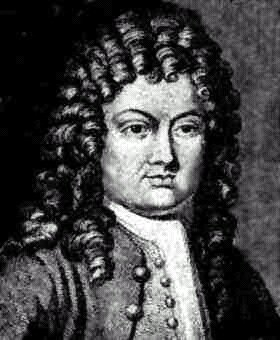
\includegraphics{numeric/figures/b_taylor}
  \caption{Brook Taylor (1685-1731)}
\end{marginfigure}

Since we only have information about the solution at discrete points, we will need to approximate the derivatives that appear in the differential equation using data from those discrete points. To write down these so--called \textbf{finite difference} approximations for derivatives, we will develop e.g. an unknown 1D function $f(x)$ in a Taylor series.

\begin{cue}
\noindent\marginnote[2.0cm]{The symbol $\mathcal{O}$ relates to the \textbf{order} of the remaining terms, i.e. how they scale as a function of $\Delta x$. Here, $\mathcal{O}\left(\Delta x^4\right)$ should really be interpreted as $\mathcal{O}\left((\Delta x)^4\right)$, i.e. if the grid size becomes twice as small, the sum of the remaining terms becomes roughly 16 times as small.}Write down Taylor expansions of $f(x+\Delta x)$ and $f(x-\Delta x)$ up till the third derivative. 
\end{cue}

\begin{gather}
f(x+\Delta x) = f(x) + \Delta x \frac{d f}{d x} + \frac{{(\Delta x)}^2}{2} \frac{d^2 f}{d x^2} + \frac{{(\Delta x)}^3}{6} \frac{d^3 f}{d x^3} + \mathcal{O}\left(\Delta x^4\right) \label{eq-taylor-plus} \\
f(x-\Delta x) = f(x) - \Delta x \frac{d f}{d x} + \frac{{(\Delta x)}^2}{2} \frac{d^2 f}{d x^2} - \frac{{(\Delta x)}^3}{6} \frac{d^3 f}{d x^3} + \mathcal{O}\left(\Delta x^4\right) \label{eq-taylor-min}
\end{gather} 

\begin{cue}
Neglecting all the terms including $\left(\Delta x\right)^2$ or higher, use Eq.~\ref{eq-taylor-plus} to approximate the first derivative of $f$.
\end{cue}

From Eq.~\ref{eq-taylor-plus} we get

\begin{equation}
\frac{d f}{d x} = \frac{f(x+\Delta x) - f(x)}{\Delta x} + \mathcal{O}\left(\Delta x\right)
\end{equation} 

This is called the \textbf{forward difference} approximation of $df / dx$. Since the error term is $\mathcal{O}(\Delta x)$, this is called a first order approximation.

\begin{cue}
Do the same, but start from Eq.~\ref{eq-taylor-min}.
\end{cue}

Similarly from Eq.~\ref{eq-taylor-min}:

\begin{equation}
\frac{d f}{d x} = \frac{f(x) - f(x- \Delta x)}{\Delta x} + \mathcal{O}\left(\Delta x\right)
\end{equation} 

This so--called \textbf{backward difference} is also first--order accurate.

\begin{cue}
Now subtract Eq.~\ref{eq-taylor-plus} and Eq.~\ref{eq-taylor-min}. What is the order of accuracy of the approximation of the derivative now? Can you explain this intuitively?
\end{cue}

By subtracting Eq.~\ref{eq-taylor-plus} and Eq.~\ref{eq-taylor-min}, we get a \textbf{central difference} formula, which now however is second--order accurate:

\begin{equation}
\fbox{$\displaystyle
\frac{d f}{d x} = \frac{f(x + \Delta x) - f(x- \Delta x)}{2 \Delta x} + \mathcal{O}\left(\Delta x^2\right)
$}
\end{equation} 

This formula is second--order accurate thanks to the cancellation of terms in the Taylor expansion. Another way of looking at is that the central difference involves not one but both neighbouring points, so it encorporates more information on the local behaviour of the function, which makes it more accurate.

Forward, backward and central differences are illustrated in Fig.~\ref{fig-fd}. From this figure, you can clearly see that the central difference is more accurate.

\begin{marginfigure}
\centering
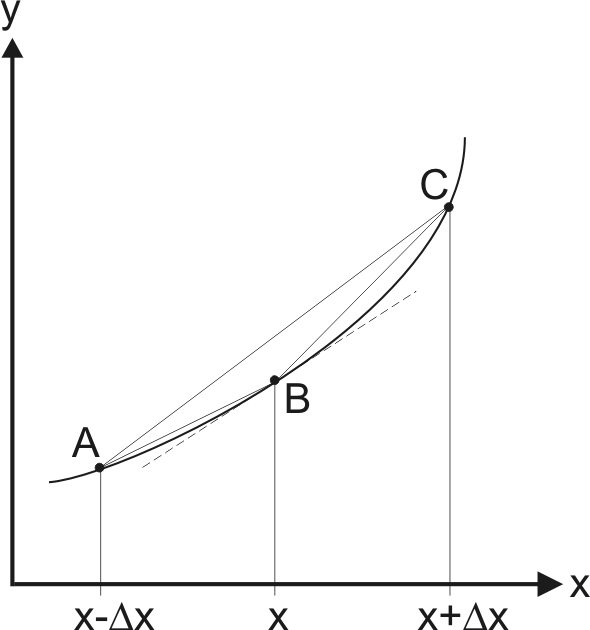
\includegraphics{numeric/figures/fd}
\caption{The arc AB represents backward differences, BC forward differences and AC central differences.}
\label{fig-fd}
\end{marginfigure}

\begin{cue}
Construct an approximation for the second derivative $f''$, this time adding Eq.~\ref{eq-taylor-plus} and Eq.~\ref{eq-taylor-min}. What is the order of approximation? 
\end{cue}

By adding Eq.~\ref{eq-taylor-plus} and Eq.~\ref{eq-taylor-min}, we get an approximation for the second derivative:

\begin{equation}
\fbox{$\displaystyle
\frac{d^2 f}{d x^2} = \frac{f(x + \Delta x) -2 f(x) + f(x- \Delta x)}{ \Delta x^2} + \mathcal{O}\left(\Delta x^2\right)
$}
\end{equation} 

If we want to get more accurate results, we could either use a finer mesh or add more information by including higher order neighbours like $f(x-2\Delta x)$ and $f(x+2\Delta x)$.

Another way of looking at the second derivative is by rewriting the approximation as

\begin{equation}
\frac{d^2 f}{d x^2} \sim  \frac{f(x + \Delta x) + f(x - \Delta x)}{2} - f(x)
\end{equation}

\noindent\marginnote{Drawing a function with an inflection point, where $f''=0$, allows you to verify that there the function is indeed equal to the average of its surroundings.}This shows that the second derivative (or the Laplacian for that matter) is all about the difference between the value of a function at a certain point and the average value of that function around that point.

\begin{marginfigure}[1.0cm]
  % credits: Wikipedia
  % url: https://en.wikipedia.org/wiki/John_Crank
  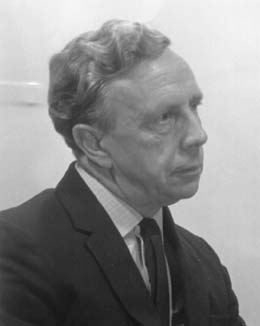
\includegraphics{numeric/figures/j_crank}
  \caption{John Crank (1916-2006)}
\end{marginfigure}

\begin{marginfigure}[8.5cm]
  % credits: Wikipedia
  % url: https://en.wikipedia.org/wiki/Phyllis_Nicolson
  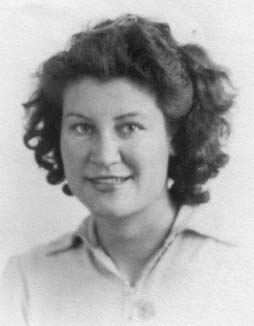
\includegraphics{numeric/figures/p_nicolson}
  \caption{Phyllis Nicolson (1917-1968)}
\end{marginfigure}

\begin{exer}
% difficulty: normal  
Construct a finite-difference scheme that will allow you to integrate the following differential equation:

$$\frac{du(t)}{dt} = -a u(t)$$

Calculate the approximations $u_n = u(n \Delta t)$ given an initial condition $u_0$ using several methods: \\

a) Approximate the time derivate using a forward difference. (This results in the forward Euler method.) \\

b) Same, but now use a backward difference. (This results in the backward Euler method.)\\

c) Construct a central difference at the intermediate time $t_{n+1/2}$ and eliminate $u_{n+1/2}$ by considering it to be the average of $u_{n}$ and $u_{n+1}$. (This results in the Crank-Nicholson method.) \\

d) Show that all of these methods can be formulated as one method (the $\theta$-rule):

$$u_{n+1} = \frac{1-(1-\theta) a \Delta t}{1+ \theta a \Delta t} u_n$$ \\

Which $\theta$-values correspond to which methods?

\end{exer}

\pagebreak

\begin{exer}
% difficulty: normal
Derive the following higher-order approximation of the second derivative:

\begin{align}  
  \frac{d^2 f}{d x^2} = \frac{1}{12 \Delta x^2} \big[& -f(x + 2 \Delta x) + 16 f(x + \Delta x) -30 f(x) \nonumber \\
  &  - f(x - 2 \Delta x) + 16 f(x- \Delta x) \big] + \mathcal{O}\left(\Delta x^4\right)
\end{align} 
\end{exer}


\pagebreak


\sectionugent{Solving the 1D wave equation with finite differences}

Illustrating finite difference methods is best done using a simple example, so we will solve the 1D Helmholtz equation in a uniform medium:

\begin{equation}
\frac{d^2 f(x)}{d x^2} + k^2 f(x) = 0 \label{eq-helmholtz-1d}
\end{equation} 

We solve this problem at a fixed wavelength, i.e. a fixed value of $k$.

\begin{cue}
  Discretise this equation.
\end{cue}

The discretised version of Eq.~\ref{eq-helmholtz-1d} reads

\begin{equation}
\frac{f(x + \Delta x) -2 f(x) + f(x- \Delta x)}{ \Delta x^2} + k^2 f(x) = 0 \label{eq-hh-diff}
\end{equation}  
 
To make this example even more concrete, let us assume a uniform grid with $\Delta x=1$ from $x=1$ to $x=5$. To illustrate boundary conditions, let us further assume that the values of $f$ are fixed at the boundaries, e.g. $f(1)=f_1$ and $f(5)=f_5$. This could be from a source forcing the electric field to a constant value, or from a metal wall which forces the electric field to zero. 

We still need to determine the following unknowns: $f(2)$, $f(3)$ and $f(4)$.


\begin{cue}
Using the discretised equation and the boundary conditions, write down 5 expressions involving $f(1)$ through $f(5)$.
\end{cue}

The discretised version of Eq.~\ref{eq-helmholtz-1d}, including the boundary conditions, reads

\begin{align}
f(1)=& \, f_1 \\
f(1) -2f(2) + f(3) + k^2 f(2) =& \, 0 \\
f(2) -2f(3) + f(4) + k^2 f(3) =& \, 0\\
f(3) -2f(4) + f(5) + k^2 f(4) =& \, 0\\
f(5)=& \, f_5
\end{align} 

Using matrix notation, this becomes

\begin{gather}
\begin{bmatrix}
1& 0& 0& 0& 0 \\
1& k^2-2& 1& 0& 0 \\
0& 1& k^2-2& 1& 0  \\
0& 0& 1& k^2-2& 1  \\
0& 0& 0& 0& 1
\end{bmatrix}
\begin{bmatrix}
f(1) \\
f(2) \\
f(3) \\
f(4) \\
f(5)
\end{bmatrix}
= 
\begin{bmatrix}
f_1 \\
0 \\
0 \\
0 \\
f_5
\end{bmatrix} \label{eq-ex-fd}
\end{gather}

So, we've reduced the problem of solving a differential equation to the problem of solving a linear system of equations of the form ${\mathbf A}\cdot{\mathbf x}={\mathbf b}$.

It is important to realise that the discretisation step that we have introduced replaces the original equation with a new one, and that even an exact solution of the discretised problem will only yield an approximate solution of the original problem. The error we have introduced in this way, is called the \textbf{discretisation error}. The hope is that by refining the mesh size, we get successively smaller discretisation errors. 


\pagebreak


%\subsection{Solving the system ${\mathbf A} \cdot {\mathbf x}={\mathbf b}$}
\sectionugent{Solving linear systems}


In order to solve the linear system ${\mathbf A}\cdot{\mathbf x}={\mathbf b}$ that arises from formulating a problem using finite differences, there are a number of options.

First of all, we can use a \textbf{direct method}, i.e. explicitly invert the matrix ${\mathbf A}$. Normally, this takes $O(N^3)$ operations, so it doesn't scale very well with large problem sizes. However, inspecting Eq.~\ref{eq-ex-fd}, we notice that the discretisation of the wave equation yields a tridiagonal matrix, where only three diagonals are non--zero. Matrix equations of this type can be solved quite efficiently, using a fairly compact variant of Gaussian elimination, taking only $O(N^2)$ operations.

A second philosophy is to give up the notion of solving the system exactly, and search for a faster approximate solution, converged relative to the discretisation error but perhaps not relative to machine round--off. This seems acceptable, especially since the algebraic equations are only an approximation to the continuum equations anyway, subject to discretisation error.

A way of constructing such an approximate solution is to use an \textbf{iterative method}: starting from an initial guess (e.g. setting all unknowns to zero), successive approximations  are constructed in the hope that after a sufficient number of iterations, the estimate converges to the true solution. There exists a plethora of literature on iterative methods, which we obviously cannot treat in detail here, but in order to get a flavour for the basic ideas, we will now discuss one of the most basic iterative schemes (which unfortunately has limited practical use in its most simple incarnation).


\pagebreak

\section{The Jacobi method}

\begin{marginfigure}[0.0cm]
  % credits: Wikipedia
  % url: https://en.wikipedia.org/wiki/Carl_Gustav_Jacob_Jacobi
  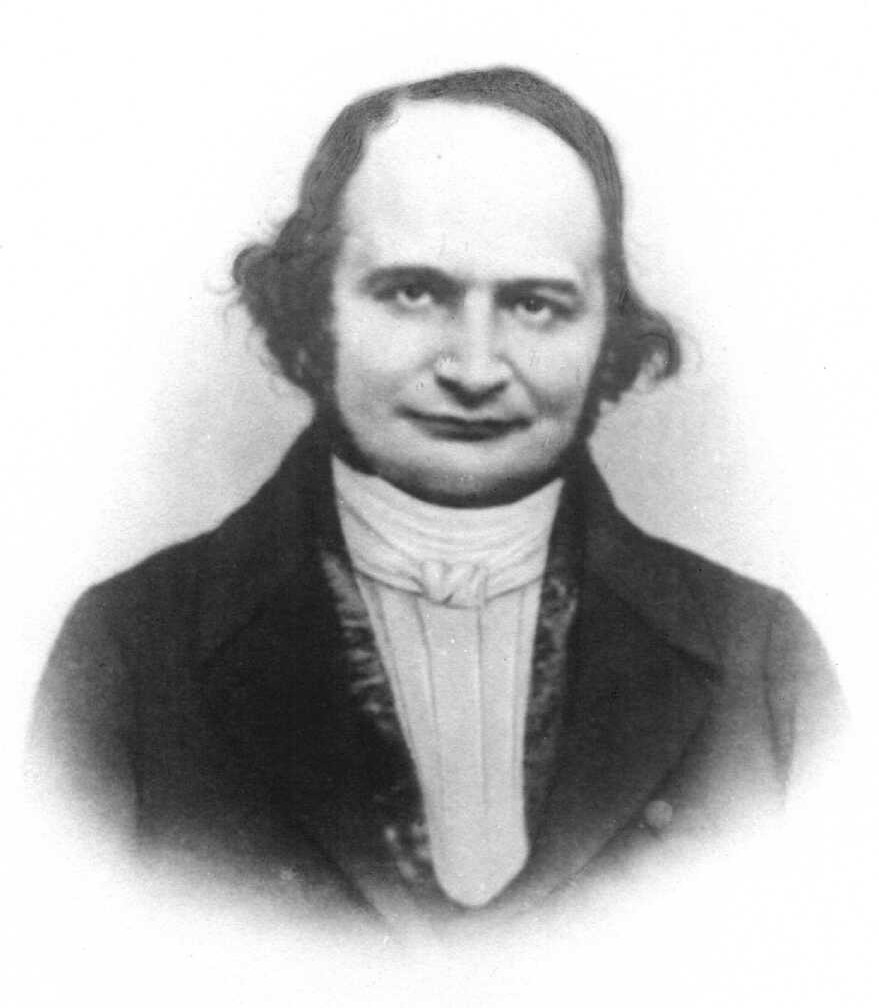
\includegraphics{numeric/figures/c_jacobi}
  \caption{Carl Gustav Jacob Jacobi (1804-1851)}
\end{marginfigure}

Let's return to the discretised version of the Helmholtz equation Eq.~\ref{eq-hh-diff}:

\begin{equation}
f_{i+1} -2 f_i + f_{i-1} +  \Delta x^2 k^2 f_i = 0 \label{eq-hh-diff-2}
\end{equation}  

The subscript $i$ denotes the values at position $x_0 + i \Delta x$.

Now, let's start from an initial set of estimates $f_i^0$, where the superscript denotes the iteration number. For Jacobi iteration, the update rule to go from estimates $f_i^n$ to $ f_i^{n+1}$ is defined as

\begin{equation}
f_{i+1}^n -2 f_i^n + f_{i-1}^n +  \Delta x^2 k^2 f_i^n = \alpha (f_i^{n+1} - f_i^n ) \label{eq-jacobi}
\end{equation}  

\begin{cue}
Have a look at this equation and try to understand why such an approach could work. What happens in case the method has found the true solution?  
\end{cue}

This can be understood as follows. If the method has converged, then the successive estimates won't change significantly anymore, such that $ f_i^{n+1} \thickapprox f_i^n $. But this means that the right--hand side of Eq.~\ref{eq-jacobi} will be equal to zero, or alternatively that $f_i^n$ is indeed the solution of Eq.~\ref{eq-hh-diff-2}.

The (positive) parameter $\alpha$ is called the relaxation parameter, which can be fine--tuned by the user of the method.

\begin{cue}
What could be advantages/disadvantages of having a small/large value of $\alpha$? 
\end{cue}

A small value of $\alpha$ means that the $f$ values will change rapidly from iteration to iteration, but with the risk of taking such large steps that the method won't converge. On the other hand, a larger value of $\alpha$ reduces the risk of diverging solutions, but on the other hand more iterations will be needed to reach convergence.

To clarify this further, we will now investigate when the Jacobi method diverges, i.e. when the $f$ values become unbounded for a bounded initial estimate.

\subsection{Convergence analysis of the Jacobi method}

To study convergence, we take an approach that is based on Fourier analysis: any wave used as the initial estimate can be written as a sum of Fourier components $e^{-j k_x x}$, which are nothing other than plane waves with wavevector $k_x$. Let's take such a plane wave and investigate what happens when iterating through the Jacobi method. If the amplitude of such a wave stays bounded when iterating, and this is true for all admissible wavevectors $k_x$, then we can be sure that whatever initial estimate will be used, the method will not produce an unbounded result at some time.

Our plane waves take the following form:

\begin{equation}
f_i^n = A^n e^{-j k_x i \Delta x}
\end{equation} 

\begin{cue}
Perform one Jacobi iteration on $f_i^n$, i.e. calculate $f_i^{n+1}$. Use that to calculate the ratio $\frac{f_i^{n+1}}{f_i^{n}}$, which will help us see whether this grows without bounds or not.  
\end{cue}

After one Jacobi iteration, we get:

\begin{equation}
f_i^{n+1} = A^n e^{-j k_x i \Delta x} \left[{ 1 + \frac{1}{\alpha}\left(e^{+ j k_x  \Delta x} - 2+  e^{-j k_x  \Delta x} + \Delta x^2 k^2\right)}\right]
\end{equation} 

or

\begin{equation}
\frac{f_i^{n+1}}{f_i^{n}} =  1 + \frac{1}{\alpha}\left[2 \cos ( k_x  \Delta x) - 2 + \Delta x^2 k^2\right]
\end{equation} 

\begin{cue}
Derive a criterion for this ratio to remain bounded, irrespective of the choice of a positive value of the relaxation parameter $\alpha$. Pay special attention to the DC component, i.e. $k=0$. 
\end{cue}

In order for this not to diverge, the ratio  $|f_i^{n+1} / f_i^{n}|$ should be smaller than 1 for any positive $\alpha$. This happens if

\begin{equation}
2 \cos ( k_x  \Delta x) - 2 \le - \Delta x^2 k^2 \label{eq-conv-jacobi}
\end{equation} 

The left--hand side of this equation lies between -4 and 0 and reaches its maximum for $k_x=0$, which is an important case as it corresponds to a uniform solution. Since it's very likely that the final solution has a DC component, we better make sure that the method converges in this case. However, for this case we can only satisfy Eq.~\ref{eq-conv-jacobi} if $k=0$. So this means that unfortunately the Jacobi method is non--convergent for the general Helmholtz equation, but only works for Laplace's equation, i.e. the special case where $k=0$.

\pagebreak

\sectionugent{Finite differences in the time domain}
\label{week6}

Without going into any detail, we finally want to mention the existence of a very popular method to solve Maxwell's equations in the time domain. This \textbf{finite--difference time--domain} method (FDTD) uses central differences to discretise the full vectorial Maxwell's equations both in space and time.

It uses a staggered grid, i.e. the electric field and the magnetic field are not discretised at the same point in space, but are arranged in a \textbf{Yee cell} (Fig.~\ref{fig-yee}). The arrangement of the field components in a Yee cell is such that the discretised curl laws of Maxwell's equations can be written out in a natural form.

\begin{figure}
\centering
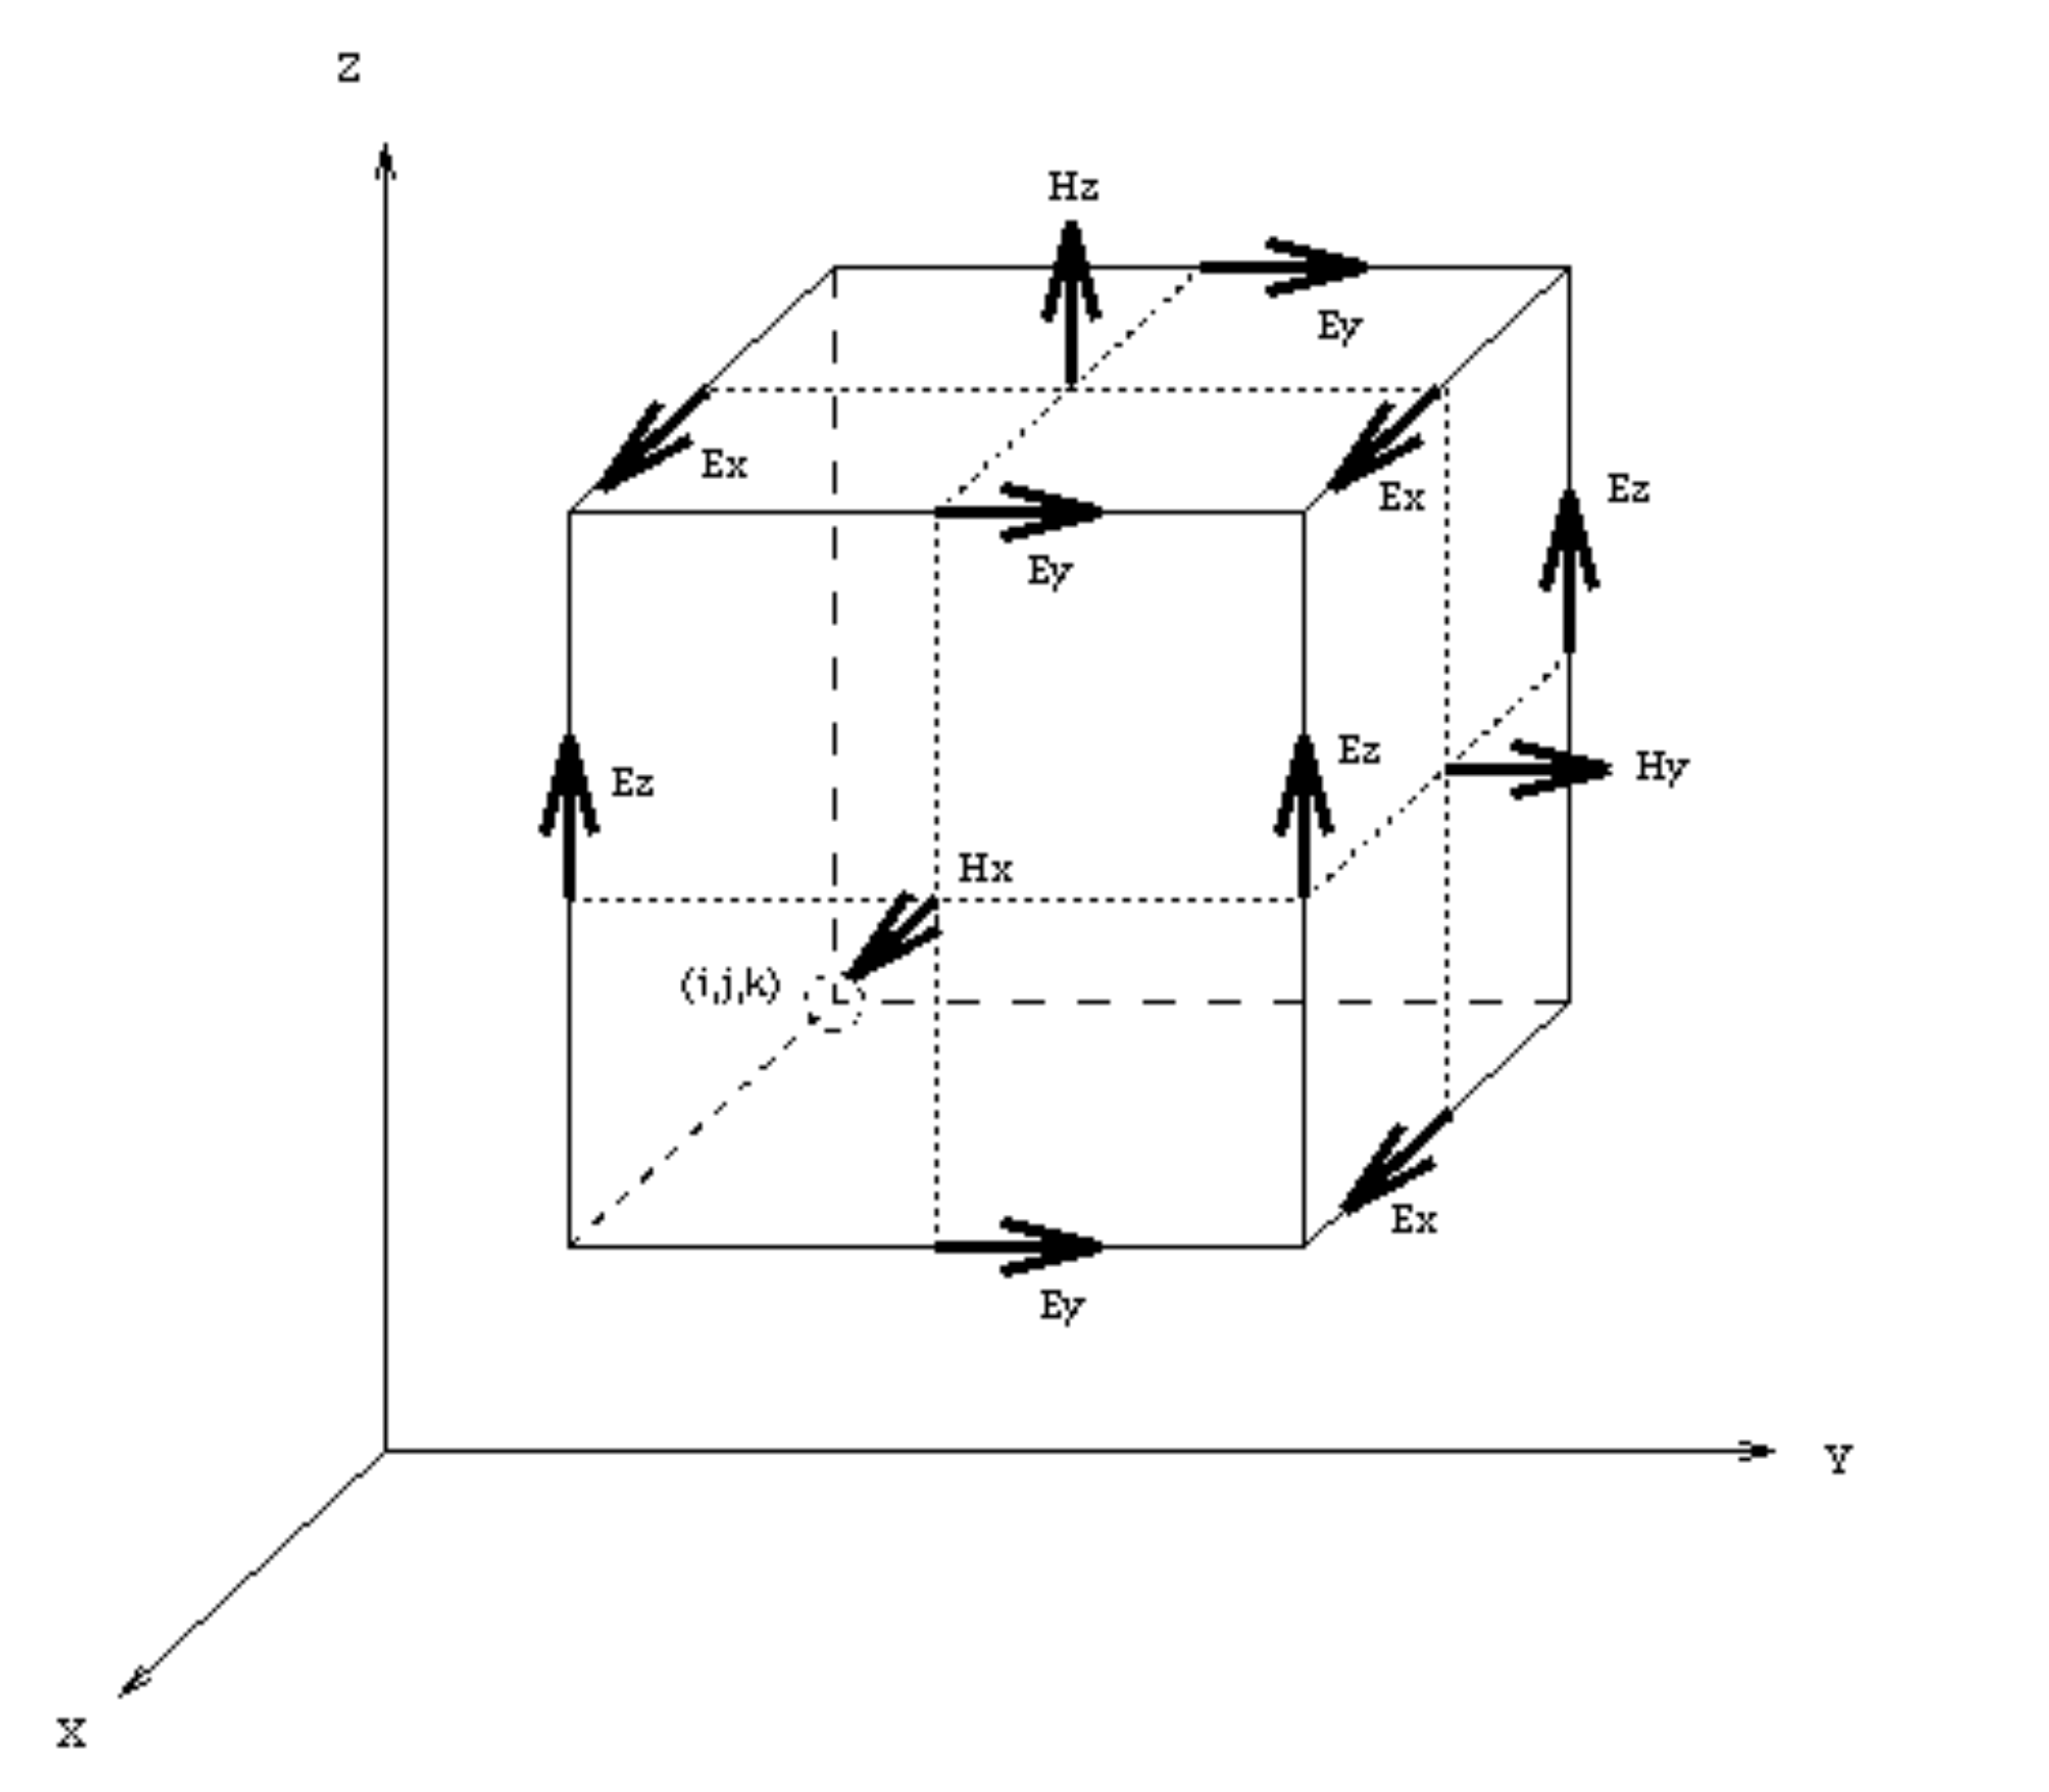
\includegraphics[width=7cm]{numeric/figures/yeecell}
\caption{The Yee cell in the FDTD algorithm.}
\label{fig-yee}
\end{figure}

As for the time evolution of the fields, FDTD uses a leap--frogging scheme, where the electric fields calculated at $t=0$ are used to determine the magnetic fields at $t=0.5$. These are subsequently used to calculate the electric fields at $t=1$ and so on.

Such a brief description obviously glosses over many important points, so consult the literature for more details.

What is important to remember though, is that this is a very general method, but the price you pay for its brute-force character is a large computational cost, combined with intrinsic errors due to the discretisation. So, always do a convergence analysis of your results as a function of the grid size.

\pagebreak

\begin{exer}
% difficulty: normal  
Use Python and its libraries NumPy and SciPy to program a finite-difference method to solve the following differential equation

$$ -\left(a(x) u'(x) \right)' + c(x)u(x) = f(x)$$

in the interval $[0,1]$, with the functions $a$, $a'$, $c$ and $f$ given, and $u(0) = u(1) = 0$. Assume that $a$ and $c$ are positive in the interval of interest.\\

Expand the derivative of the product, and use a backward-difference approximation for $u'$ and a central-difference approximation for $u''$. \\

Use a sparse solver to take advantage of the banded matrix structure. Consult the SciPy documentation for the right way to construct these matrices. \\

To check your results, try the solver using the following set of functions:

$$a_1(x) = 1 + x^2$$
$$c_1(x) = 0$$
$$u_1(x) = x(1-x) e^x $$

To do so, construct the required $f(x)$ from $a_1(x)$, $c_1(x)$ and the exact solution $u_1(x)$ and evaluate how close the numerical approximation of $u$ is to this analytical form.

\end{exer}



\pagebreak


\sectionugent{Basic recipe for finite elements}

All finite element methods more or less share the same philosophy, which is outlined in the following recipe:

\begin{itemize}
\item

\begin{marginfigure}
\centering
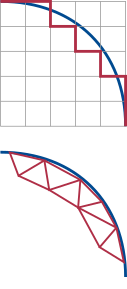
\includegraphics[width=3cm]{numeric/figures/staircase}
\caption{A triangular mesh follows a curved boundary much better than a square grid.}
\label{fig-staircasing}
\end{marginfigure}

\begin{marginfigure}
\centering
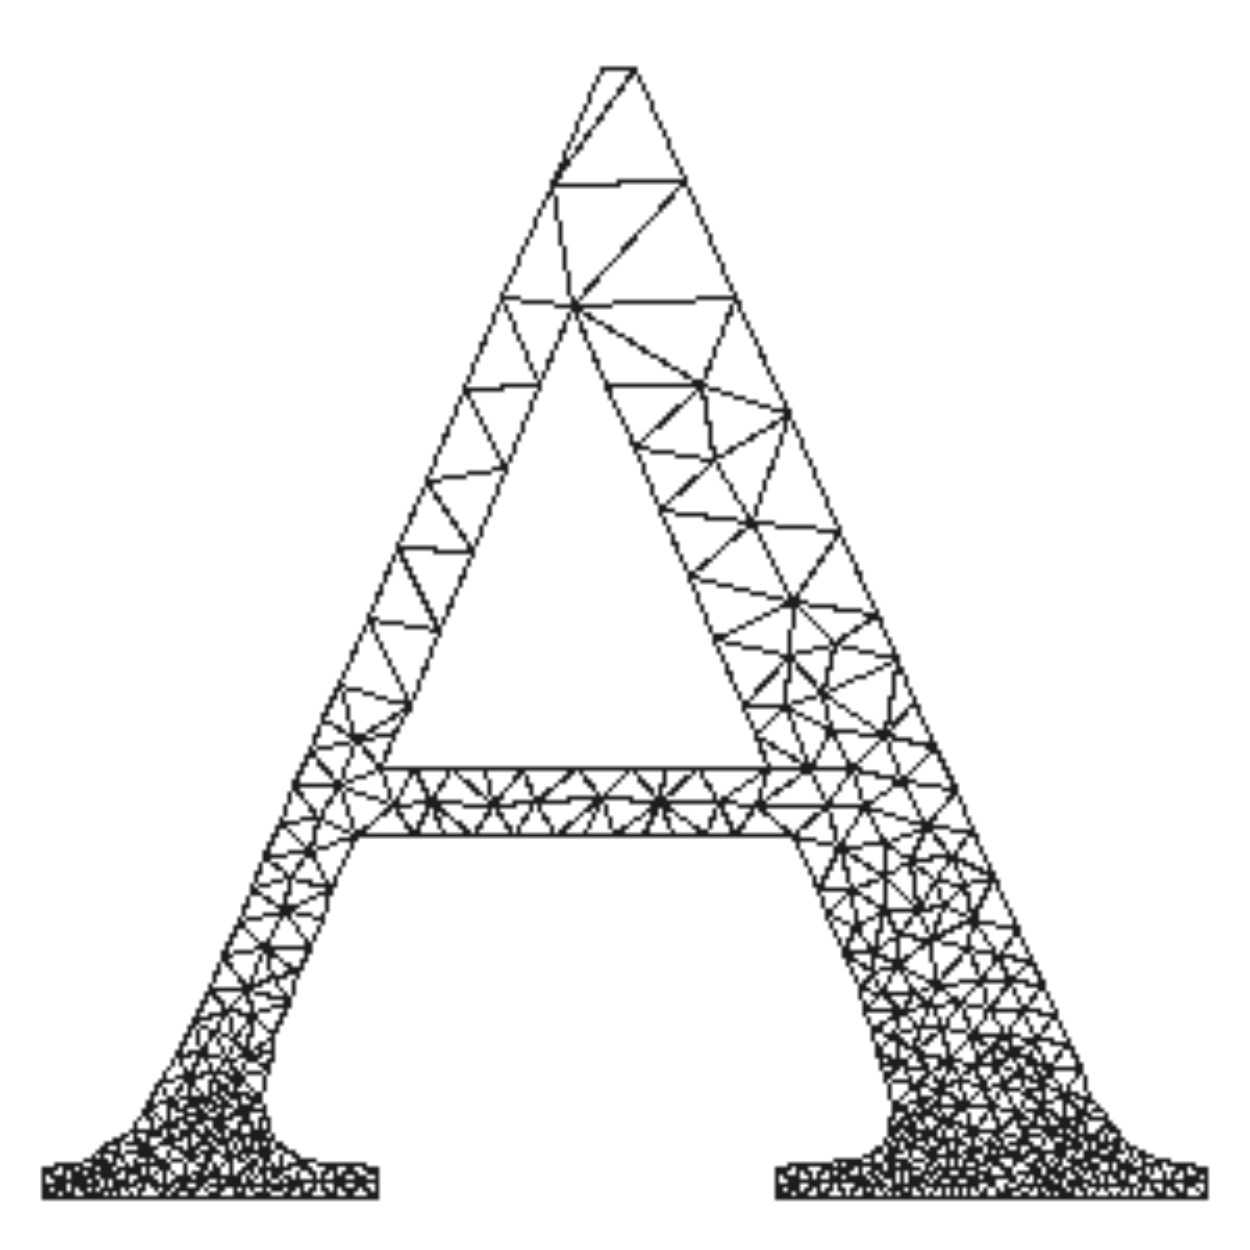
\includegraphics[scale=0.5]{numeric/figures/grid}
\caption{A triangular mesh can be locally refined.}
\label{fig-grid}
\end{marginfigure}



Subdivide the structure you want to model into $K$ finite subsections (hence the name finite elements). The elements don't have to be the same size, the mesh can be irregular. A triangular mesh is a popular choice, because this allows one to approximate curved boundaries much better than e.g. with the rectangular grid that was used in finite difference methods (Fig.~\ref{fig-staircasing}). An additional advantage is that you can use more triangles are used where higher resolution is required (Fig.~\ref{fig-grid}). Such a local refinement of the grid turns out to be much more complicated in a finite-difference method.
  

\item
Approximate the unknown function using a separate approximation expression for each element of the form
\begin{equation}
\psi(x,y) = \sum_{i=1}^M u_i b_i(x,y) \label{eq-fe-1}
\end{equation}

Here the $b_i(x,y)$ are some convenient set of known basis functions. In order to solve the problem, the $M$ unknown coefficients $u_i$ per element still need to be determined.
\item
  Introduce some constraint on the $MK$ number of unknowns, e.g. to ensure that $\psi$ is continuous across the elements.



\item
Write down an expression $J$ containing the approximating functions $b_i$ and the coefficients $u_i$. Because the $b_i$ are chosen in advance and therefore known, $J$ is function of the unknown $u_i$ only. The precise form of $J$ differs from problem to problem, but is often related to the total energy in the system.
\item
Find the coefficients $u_i$ such that $J$ is minimised. In a popular method due to \textbf{Rayleigh and Ritz}, this is done simply by setting all $\partial J / \partial u_i$ equal to zero and solving the resulting linear system. If $J$ is an expression for the total energy in the system, there is a clear physical interpretation for this procedure: the true solution to the problem is one that minimises the energy in the system.
\end{itemize}


\pagebreak


\sectionugent{Solving the 1D wave equation with finite elements}

\begin{marginfigure}[0.5cm]
  % credits: Wikipedia
  % url: https://en.wikipedia.org/wiki/John_William_Strutt,_3rd_Baron_Rayleigh
  \includegraphics{numeric/figures/Rayleigh}
  \caption{John William Strutt, 3rd Baron Rayleigh (1842-1919)}
\end{marginfigure}

In order to make the recipe from the previous section more concrete, we will now indicate in more detail how finite element methods can be used to solve the 1D Helmholtz equation in a uniform medium, i.e. the same problem we used to illustrated the concept of finite differences:

\begin{equation}
\frac{d^2 \psi (x)}{d x^2} + k^2 \psi(x) = 0 \label{eq-helmholtz-1d-2}
\end{equation} 

\subsection{Piecewise approximation}

To describe the unknown function $\psi$, we will use a very simple but common approach, which is that of a piecewise straight approximation. We will subdivide our domain into $K$ finite elements being line segments of identical length. In each segment, we will assume that $\psi$ varies linearly between the end points $x_1$ and $x_2$ of that segment:

\begin{equation}
\psi(x) = \frac{x_2 - x}{x_2 - x_1} \psi_1 + \frac{x - x_1}{x_2 - x_1} \psi_2 \label{eq-fe-2}
\end{equation} 

Here $\psi_1$ and $\psi_2$ are the so far unknown values of $\psi$ at $x_1$ and $x_2$ respectively. End points of the segments are often called \textbf{nodes} of the mesh.

\begin{cue}
Looking at Eq.~\ref{eq-fe-2}, what would be the set of basis functions we use in this case?
\end{cue}

Comparing Eq.~\ref{eq-fe-1} and \ref{eq-fe-2}, we get that $M=2$, $u_i$ is $\psi_i$ and

\begin{align}
b_1(x) =& \, \frac{x_2 - x}{x_2 - x_1} \\
b_2(x) =& \, \frac{x - x_1}{x_2 - x_1}
\end{align} 

\begin{marginfigure}
\centering
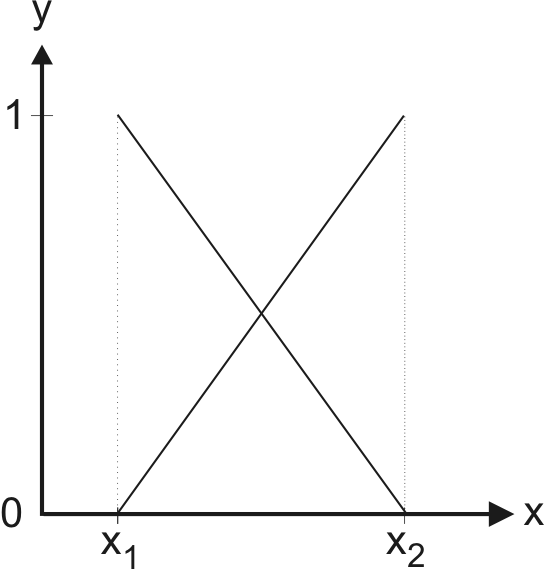
\includegraphics{numeric/figures/interpol}
\caption{Simple shape functions $b_1(x)$ and $b_2(x)$ for a 1D finite element model.}
\label{fig-shape}
\end{marginfigure}

These shape functions or interpolation functions are sketched in Fig.~\ref{fig-shape}.

(It is sometimes useful to express the interpolation functions in terms of a local scaled coordinate $\xi=(x-x_1)/(x_2-x_1)$ ranging from 0 to 1. The advantage of local coordinates is that expressions for $J$ can be more easily applied to the case where the size of the elements is not the same throughout the mesh.)

\subsection{Joining the elements}

The elements are not independent but are usually coupled through some continuity condition. In the case of our problem, $\psi$ needs to be continuous across elements. The effect of this is that the number of unknowns is reduced.

To see how this is done in practice, consider Fig.~\ref{fig-connect}  with on one hand a \textbf{disconnected} local numbering scheme of the nodes, and on the other hand a \textbf{connected} global numbering scheme, which already takes the continuity conditions into account.

\begin{marginfigure}
\centering
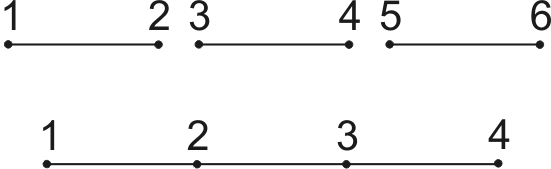
\includegraphics{numeric/figures/connect}
\caption{\textbf{Top}: disconnected local numbering. \textbf{Bottom}: connected global numbering.}
\label{fig-connect}
\end{marginfigure}

\begin{cue}
For the example in Fig.~\ref{fig-connect}, use a matrix to express the relation between $\psi_{i, \mathrm{disc}}$ in the disconnected numbering scheme and  $\psi_{i, \mathrm{con}}$ in the connected numbering scheme.
\end{cue}
  
The disconnected values are related to connected values by the following matrix equation:

\begin{equation}
\begin{bmatrix}
\psi_1 \\ \psi_2 \\ \psi_3 \\ \psi_4 \\ \psi_5 \\ \psi_6
\end{bmatrix}_{\mathrm{disc}}
=
\begin{bmatrix}
1 & 0 & 0 & 0  \\ 
0 & 1 & 0 & 0  \\   
0 & 1 & 0 & 0  \\ 
0 & 0 & 1 & 0  \\   
0 & 0 & 1 & 0  \\  
0 & 0 & 0 & 1  
\end{bmatrix}
\begin{bmatrix}
\psi_1 \\ \psi_2 \\ \psi_3 \\ \psi_4
\end{bmatrix}_{\mathrm{con}}
\label{eq-con-matrix}
\end{equation} 

The matrix in Eq.~\ref{eq-con-matrix} is called the \textbf{connection matrix} of the mesh. Obviously, for such a simple case is seems overkill to write the continuity equations in matrix form, but for complicated 3D meshes such a matrix has its practical value for computer implementation of finite element methods.

\subsection{An expression for $J$}

In order to keep the method physically interpretable, let's use the total energy of the system as an expression for $J$. Assume that each element has constant refractive index. From the complex Poynting theorem, we know that the time--averaged stored energy in a system is given by

\begin{align}
J =& \, \frac{1}{2} \int ( {\mathbf E} \cdot {\mathbf D}^* - {\mathbf H} \cdot {\mathbf B}^* ) dx \\
  =& \, \frac{1}{2} \int ( \varepsilon |{\mathbf E}|^2 - \mu |{\mathbf H}|^2 ) dx
\end{align} 

\begin{cue}
Use Maxwell to eliminate ${\mathbf E}$ from that expression. Then, simplify it for the TM case where ${\mathbf H} = H {\mathbf 1}_z = \psi {\mathbf 1}_z $.  
\end{cue}

We can use one of Maxwell's curl laws to eliminate ${\mathbf E}$:

\begin{equation}
{\mathbf E} = \frac{1}{j \omega \varepsilon} \nabla \times {\mathbf H}
\end{equation}  

Let's assume that we are working in the TM case, where ${\mathbf H} = H {\mathbf 1}_z = \psi {\mathbf 1}_z $. We get

\begin{equation}
J = \frac{1}{2} \int \left( \frac{1}{\omega ^2 \varepsilon}\left|{\frac{d H}{d x}}\right|^2 - \mu |H|^2 \right) dx
\end{equation}

Although we will not prove it here, it can be shown that in the case of lossless media, we can always scale the solution such that the absolute values in the previous equation can be replaced by simple squares. Also, multiplying $J$ by the constant $2 \omega ^2 \varepsilon$ does not affect the location of the minimum, such that finally we can write

\begin{equation}
J = \int \left( \left(\frac{d H}{d x}\right)^2 - k^2 H^2 \right) dx
\end{equation}

or going back to our function $\psi$:

\begin{equation}
\fbox{$\displaystyle
J = \int \left( \left(\frac{d \psi}{d x}\right)^2 - k^2 \psi^2 \right) dx \label{eq-J-power}
$}
\end{equation} 

The contribution of a single element to $J$ can now be calculated in terms of the unknown nodal values $\psi_i$ using the explicit form of the shape functions from Eq.~\ref{eq-fe-2}. This leads to tedious but straightforward algebra, which we will not repeat here. In view of the structure of Eq.~\ref{eq-J-power}, the contribution of a single element leads to a bilinear equation of the form

\begin{equation}
J_i = \begin{bmatrix}
\psi_1 \psi_2 
\end{bmatrix}_{disc}
\begin{bmatrix}
A & B \\
C & D 
\end{bmatrix}
\begin{bmatrix}
\psi_1 \\ \psi_2
\end{bmatrix}_{disc}
\label{eq-J-power-i}
\end{equation} 

The total energy is just the sum of the contributions from all elements, which can also be cast in matrix form, this time with a block diagonal matrix, each block corresponding to a matrix of the type from Eq.~\ref{eq-J-power-i}.

\begin{exer}
% difficulty: trivial
Explicitly write down this total energy $\sum J_i$ using a block diagonal matrix.
\end{exer}

Finally, the expressions in terms of disconnected nodal values can be transformed in terms of connected values using the connection matrix, like e.g. the one from Eq.~\ref{eq-con-matrix}. In this way, all the continuity conditions are imposed.

\subsection{Minimising $J$}

To find the unknowns $\psi_i$ that minimise $J$ we simply impose

\begin{equation}
\frac{\partial J}{\partial \psi_i} = 0 \label{eq-rayleigh-ritz}
\end{equation} 

and this for all $i$. Since $J$ is a bilinear form, Eq.~\ref{eq-rayleigh-ritz} takes the form of $MK$ linear equations with $MK$ unknowns. Just as was the case with the finite--difference method, this system can either be solved directly or iteratively.


\pagebreak


\sectionugent{Finite elements as a variational method}

In theory, the outline of the finite element method that we have given so far is perfectly adequate to describe it. However, it yields additional insight to cast it in the framework of a variational method.

Before doing that, let's recap same well-known facts, but in such a way that will make it easier for us to generalise to the new terminology.

A function $f(x)$ of one variable takes a number $x$ as input, and delivers another number as output. Suppose this function has a minimum for some value of $x$. At that point, the output of the function does not change to first order, i.e. $\delta f=0$ for all possible directions $\delta x$ around that point. Obviously, in this 1D case, there are only two trivial directions, i.e. $+x$ and $-x$.

A function $f(x,y)$ of two variables takes two numbers $x$ and $y$ as input, and spits out another number as output. Also here, when there is a minimum, the output of the function does not change, i.e. $\delta f=0$ for all possible directions  $\delta x \mathbf{1}_x  + \delta y\mathbf{1}_y$ you might explore in the neighbourhood of the minimum.

\begin{marginfigure}[-1.5cm]
  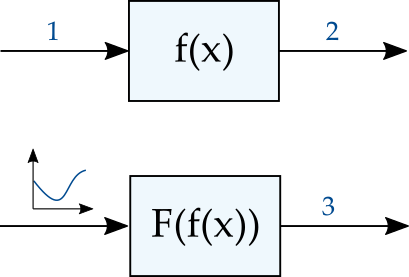
\includegraphics{numeric/figures/function_functional}
  \caption{Function vs. functional}
  \label{fig-function-functional}
\end{marginfigure}

Now, let's introduce a \textbf{functional}. This is an object $F(f(x))$ that consumes as input a function $f(x)$ and delivers a number as output (Fig.~\ref{fig-function-functional}). In contrast to functions, you could say that the input of a functional is not finite dimensional, but infinite dimensional, as it takes an infinite set of numbers to specify an arbitrary function. All of these objects however have a single number as output.

\begin{cue}
Can you think of examples of a functional?  
\end{cue}

The entity $J$ that we have introduced in this chapter is a functional, as it maps a function $\psi$ to a scalar (being in this case the energy of the system), so $E=J(\psi)$. (Nitpicking: in applying the Rayleigh--Ritz method, we have parametrised the function $\psi$ using a finite set of unknowns $\psi_i$. This effectively turns the functional $J(\psi)$ into a vanilla function $J(\psi(\psi_i))$, albeit one of multiple arguments.)

\begin{exer}
  % difficulty: trivial
  % ugent
  % youtube: gbKEmkNIA6k
  Function or functional?

  a) $f(x)=\int_0^x t^2 dt$

  b) $f(x)=\int_0^1 x^2(t) dt$
  \begin{sol}
    a) function b) functional
  \end{sol}
\end{exer}

A \textbf{variational expression} comes from minimising a functional over a set of admissible functions. Indeed, every input $\psi$ to the functional will result in a different number $J(\psi)$ at the output, and we are looking for the special $\psi$ that will result in the smallest possible output.

In the case of finite elements, we have been solving the following variational expression:

\begin{equation}
E = \min_\psi J(\psi)
\end{equation} 

where $E$ is the total energy in the system, and $\psi$ are functions coming from an admissible set, e.g. continuous functions that satisfy the boundary conditions of the problem.

\begin{marginfigure}[-1.5cm]
  % credits: Wikipedia
  % url: https://en.wikipedia.org/wiki/Walther_Ritz
  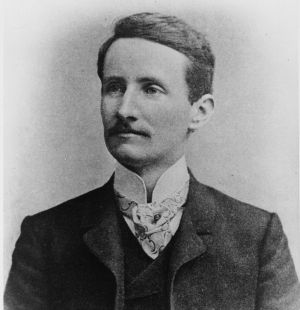
\includegraphics{numeric/figures/w_ritz}
  \caption{Walther Ritz (1878-1909)}
\end{marginfigure}

The \textbf{Rayleigh--Ritz} method to minimise a functional is to expand $\psi$ in a finite number of known basis functions, and then determine the expansion coefficients such that the functional is minimised. This turns the infinite-dimensional problem into a much more tractable finite-dimensional one.

\begin{cue}
What can you say about the sensitivity of $E$ to e.g. rounding errors, given that we are working at the minimum of the functional? 
\end{cue}

\begin{marginfigure}[1.5cm]
  \includegraphics{numeric/figures/minimum}
  \caption{A function (or functional) does not vary to first order at its minimum.}
  \label{fig-functional-min}
\end{marginfigure}

So far, we don't seem to have done anything useful except introducing some new terminology. However, by looking at the energy $E$ as a minimum of a functional, we realise that a small variation $\delta \psi$ (caused e.g. by numerical round--off errors) will not have a very big impact on the calculated value of $E$, since $\delta J=0$ at the minimum of the functional, for all possible 'directions' $\delta \psi$. This insensitivity to errors is a big bonus for practical applications, and means that methods which have a variational basis can be much more robust.

Now, the energy $E$ is a decidedly uninteresting quantity for practical applications, so the fact that we can calculate it without being very sensitive to rounding errors is of limited use. However, it is possible to derive variational expressions for e.g. the propagation constant of a waveguide, which is a much more relevant parameter that people are interested in.

\pagebreak


\sectionugent{Variational form for the 3D Helmholtz equation}

In this section, we wish to provide some extra proof that a function that minimises the functional from Eq.~\ref{eq-J-power} is indeed a solution to the Helmholtz equation. So far, this was only made acceptable by invoking physical arguments based on minimum energy, but a mathematical proof for this was lacking. At the same time, let's extend the method to three dimensions:

\begin{equation}
J = \iiint \left((\nabla \psi)^2 - k^2 \psi^2 \right) dV \label{eq-variational1}
\end{equation} 

\noindent\marginnote{$\delta J=0$ can obviously also give us a maximum, but these situations are rare in practice and can be easily identified by exploring $J$ in the neighbourhood of the potential solution.}If a function $\psi$ minimises the functional $J$, then $\delta J$ has to be zero for $\psi$.

\begin{cue}
Calculate $\delta J$ for this functional, neglecting second-order terms in $\delta \psi$.
\end{cue}

\noindent\marginnote[3.3cm]{Don't get confused: $\left( \nabla \psi \right)^2 = \nabla \psi \cdot \nabla \psi \ne \nabla^2 \psi $}For $\delta J$ (also called the \textbf{first variation} of $J$) we get

\begin{align}
\delta J =& \, J(\psi + \delta \psi) - J(\psi) \nonumber \\
  =& \, \iiint \left( (\nabla (\psi + \delta \psi))^2 - k^2 (\psi + \delta \psi)^2 \right) dV \nonumber   \\
  -& \, \iiint \left((\nabla \psi)^2 - k^2 \psi^2 \right) dV
\end{align} 

If we neglect second-order terms in $\delta \psi$, we get

\begin{equation}
\delta J = \iiint \left( 2 \nabla \psi \cdot \nabla (\delta \psi) - 2 k^2 \psi \delta \psi \right) dV
\end{equation}

Now, let's make use of the following vector identitity:

\begin{equation}
\nabla \cdot (u \nabla v) = u \nabla \cdot \nabla v + (\nabla u) \cdot (\nabla v) \label{eq-vector-id-green-other}
\end{equation} 

\begin{cue}
Take the volume integral of this identity and apply the divergence theorem. Next, use this expression to transform $\delta J$. Figure out how to best assign $u$, $v$ to $\psi$, $\delta \psi$, bearing in mind that the ultimate goal is to bring out the Helmholtz equation.
\end{cue}

By integrating Eq.~\ref{eq-vector-id-green-other}, we actually get one of the many incarnations of Green's theorem:

\begin{equation}
\iiint \nabla \psi \cdot \nabla (\delta \psi) dV = \iint \delta \psi \cdot \frac{\partial \psi}{\partial n} dS - \iiint \delta \psi \cdot \nabla^2 \psi dV
\end{equation} 

So,

\begin{equation}
\delta J = 2\iint \delta \psi \cdot \frac{\partial \psi}{\partial n} dS - 2\iiint \delta \psi \cdot \nabla^2 \psi dV - 2 \iiint k^2 \psi \delta \psi dV
\end{equation} 

\begin{cue}
Now, impose the condition that says that $\psi$ should minimise $J$.  
\end{cue}

Demanding that $\delta J = 0$ (a condition which is called \textbf{stationarity}), we get

\begin{equation}
\iiint \delta \psi (\nabla^2 \psi + k^2 \psi ) dV = \iint \delta \psi \cdot \frac{\partial \psi}{\partial n} dS \label{eq-euler-lagrange-1}
\end{equation}

\begin{cue}
Think about how to deal with the term involving the boundary condition, i.e. the 2D integral.  
\end{cue}

\begin{marginfigure}[0.0cm]
  % credits: Wikipedia
  % url: https://en.wikipedia.org/wiki/Peter_Gustav_Lejeune_Dirichlet
  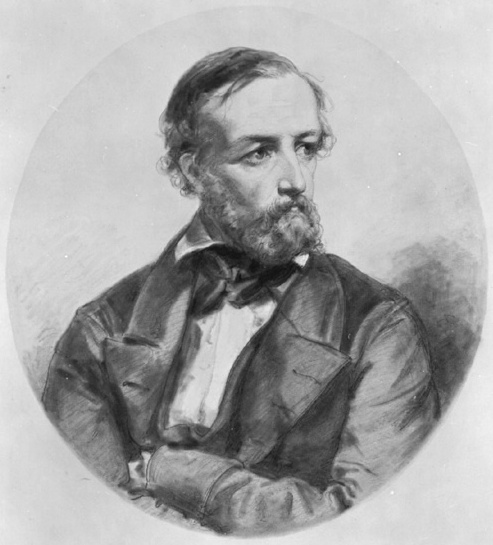
\includegraphics{numeric/figures/p_dirichlet}
  \caption{Peter Gustav Lejeune Dirichlet (1805-1859)}
\end{marginfigure}

Suppose that our boundary conditions are of the Dirichlet type such that $\psi=0$ on the boundary. In other words, we are restricting our search to only include functions that vanish at the boundary. Then, in order to be an admissible function that satisfies the boundary condition, $\delta \psi$ also has to be zero on the boundary, so that the right--hand side of Eq.~\ref{eq-euler-lagrange-1} will be zero.

Similarly, for Neumann--type boundary conditions where $\partial \psi / \partial n = 0$ on the boundary, the right--hand side of Eq.~\ref{eq-euler-lagrange-1} will also be zero.

So for these common boundary conditions we get

\begin{equation}
\iiint \delta \psi (\nabla^2 \psi + k^2 \psi ) dV = 0
\end{equation} 

Since our choice of $\delta \psi$ has been completely arbitrary, it follows that stationarity of the variational expression requires that $\psi$ has to satisfy

\begin{equation}
\nabla^2 \psi + k^2 \psi = 0 \label{eq-euler-lagrange-2}
\end{equation} 

This is of course the Helmholtz equation.

Eq.~\ref{eq-euler-lagrange-2} is called the \textbf{Euler} or the \textbf{Euler--Lagrange} equation of the variational formulation Eq.~\ref{eq-variational1}.


\begin{exer}
% difficulty: trivial
% ugent
% youtube: qM9NOykRESw
Show that demanding that the 1D Helmholtz equation is orthogonal to any arbitrary function leads to the variational form 

$$J = \int \left( \left(\frac{d \psi}{d x}\right)^2 - k^2 \psi^2 \right) dx$$

\end{exer}


\begin{exer}
% difficulty: normal
  
Construct the best least-squares approximation to the parabola 

$$f(x) = 10(x-1)^2 -1$$ 

in the interval $[1,2]$ using only functions from $V = \mathrm{span} \{1, x\}$.

\begin{sol}
$$f(x) = 10(x-1)^2 -1$$   
\end{sol}
\end{exer}


\begin{exer}
% difficulty: normal
% ugent
% youtube: cHTTlU_ewds
  
  Consider an arbitrarily shaped waveguide filled with air but bounded by perfectly conducting metal walls.

  a) Show that the eigenmodes of the waveguide, i.e. solutions which have a $z$-dependence of $\exp{(-j k_z z)}$, satisfy the following equation:

$$ \nabla_{xy}^2 \psi + \left( k^2 - k_z^2 \right)\psi = 0 $$ 

Here, $\nabla_{xy}$ is the transverse differential operator, which does not contain derivatives in the $z$-direction.

\noindent\marginnote{Note the difference between this cut-off condition for closed metal wave-guides and the one for open wave-guides, which is $k=k_{\mathrm{clad}}$} b) We are interested in finding the value of $k$ at cut--off ($k_z^2=0$), because we can get the cut-off wavelength from that. Show that the following is a variational expression for this cut--off wavevector $k_{\mathrm{cut}}$:

$$ k_{\mathrm{cut}}^2 = \frac{\iint_S (\nabla_{xy} \psi)^2 dS}{\iint_S \psi^2 dS}$$

Here $S$ is the cross--section of the waveguide.

c) Looking back at Eq.~\ref{eq-variational1}, what can you say about the energy of such a mode at cut-off?

\end{exer}

\pagebreak

% Sorry Leonard, no space here.

%\begin{marginfigure}[3.0cm]
  % credits: Wikipedia
  % url: https://en.wikipedia.org/wiki/Leonhard_Euler
%  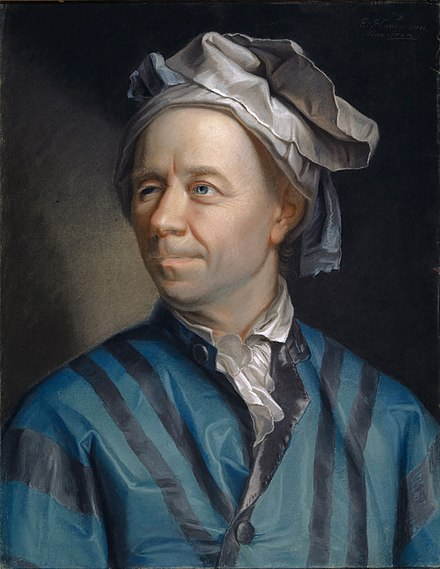
\includegraphics{numeric/figures/l_euler}
%  \caption{Leonhard Euler (1707-1783)}
%\end{marginfigure}

\begin{marginfigure}[1.0cm]
  % credits: Wikipedia
  % url: https://en.wikipedia.org/wiki/Joseph-Louis_Lagrange 
  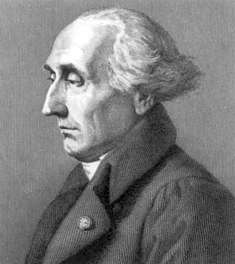
\includegraphics{numeric/figures/j_lagrange}
  \caption{Joseph-Louis Lagrange (1736-1813)}
\end{marginfigure}


\begin{exer}
% difficulty: normal
Use the identity

$$\iint_S p \nabla q \cdot \nabla r dS= - \iint_S q \nabla \cdot (p \nabla r) dS + \int_{\delta S} pq \frac{\partial r}{\partial n} dl$$

to find the Euler-Lagrange equation of the following variational expression

$$J(\phi)=\iint_S f(x,y) (\nabla \phi)^2 dS$$

with $f(x,y)$ a given scalar function.

\begin{sol}
$$\nabla \cdot \left( f \nabla \phi \right) = 0 $$
\end{sol}
\end{exer}


\pagebreak


\sectionugent{Eigenmode expansion}
\label{week7}

In eigenmode expansion, we slice up the structure that we want to model in a number of layers where the refractive index profile does not change in the propagation direction (often taken to be the $z$--direction). A typical example is given in Fig.~\ref{fig-interface}, which shows the interface between two waveguides I and II.

\begin{figure}[ht]
\centering
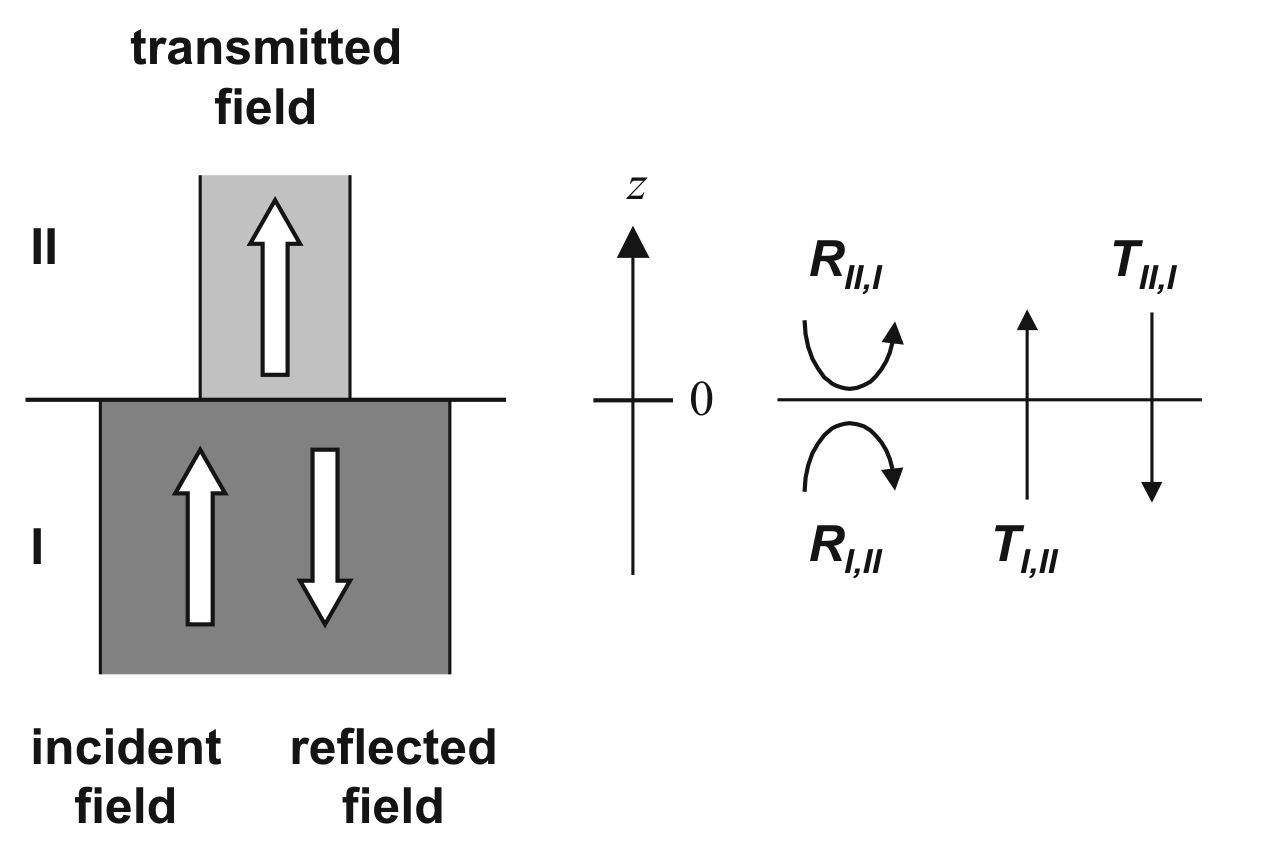
\includegraphics{numeric/figures/interface}
\caption{Interface between two layers.}
\label{fig-interface}
\end{figure}

We will expand the field in each waveguide using the eigenmodes of that waveguide. It can be shown that these eigenmodes form a \textbf{complete} set, i.e. they can be used to expand any arbitrary field in that layer. Also, by enclosing the structure that we want to model in a metal box, this set of eigenmodes is a discrete set rather than a continuum.

The interface is placed at $z=0$ and a single mode with index $p$ is incident from medium I. This incident mode will give rise to a backward--propagating field in medium I, which we expand in terms of the eigenmodes of this medium. Likewise, we expand the transmitted field in the eigenmodes of medium II.

Before continuiting, we need to determine a relationship between the fields of the forward and the backward propagating modes.

\begin{exer}
% difficulty: trivial
Assume you solve Maxwell's equations to find a certain eigenmode solution, i.e. a solution with a $z$-dependence of $\exp{(-j \beta z)}$. Let's say this solution is characterised by the following tangential ($x$ and $y$) and normal ($z$) components:

$$\left( \mathbf{E}_{t},\mathbf{E}_{z},\mathbf{H}_{t},\mathbf{H}_{z},\beta \right)$$

By writing down the different components of Maxwell's curl equations, show that there also exists another solution:

$$  \left( \mathbf{E}_{t},-\mathbf{E}_{z},-\mathbf{H}_{t},\mathbf{H}_{z},-\beta \right) $$

Because of the negative propagation constant, this is the backward propagating version of the same eigenmode.

\end{exer}

Now that we know this, we can start applying the well--known \textbf{mode--matching} technique.

\begin{cue}
Impose the continuity of the tangential components of the total field on both sides of the interface in Fig.~\ref{fig-interface}.  
\end{cue}

Demanding continuity leads to: 

\begin{eqnarray}
\mathbf{E}^{I}_{p,t}+\sum _{j}R_{j,p}\mathbf{E}^{I}_{j,t} & = & \sum _{j}T_{j,p}\mathbf{E}^{II}_{j,t}\label{Eq:MM 1a} \\
\mathbf{H}^{I}_{p,t}-\sum _{j}R_{j,p}\mathbf{H}^{I}_{j,t} & = & \sum _{j}T_{j,p}\mathbf{H}^{II}_{j,t}\label{Eq:MM 1b} 
\end{eqnarray}

(The minus sign for the reflected tangential ${\mathbf H}$ field comes from the explicit form of the backward eigenmode we derived above.)

To calculate the unknown expansion coefficients $R_{j,p}$ and $T_{j,p}$ (which can be seen as reflection and transmission coefficients), we take the right cross product of Eq.~\ref{Eq:MM 1a} with $\mathbf{H}^{I}_{i,t}$ and the left cross product of Eq.~\ref{Eq:MM 1b} with $\mathbf{E}^{I}_{i,t}$. Here, $i$ is an arbitrary index. Afterwards, we integrate over the cross--section.

\begin{cue}
  Perform these operations.
\end{cue}

We get:

\begin{eqnarray}
\left\langle \mathbf{E}^{I}_{p},\mathbf{H}^{I}_{i}\right\rangle +\sum _{j}R_{j,p}\left\langle \mathbf{E}^{I}_{j},\mathbf{H}^{I}_{i}\right\rangle  & = & \sum _{j}T_{j,p}\left\langle \mathbf{E}^{II}_{j},\mathbf{H}^{I}_{i}\right\rangle \label{Eq:MM 2a} \\
\left\langle \mathbf{E}^{I}_{i},\mathbf{H}^{I}_{p}\right\rangle -\sum _{j}R_{j,p}\left\langle \mathbf{E}^{I}_{i},\mathbf{H}^{I}_{j}\right\rangle  & = & \sum _{j}T_{j,p}\left\langle \mathbf{E}^{I}_{i},\mathbf{H}^{II}_{j}\right\rangle \label{Eq:MM 2b} 
\end{eqnarray}

where the scalar product is defined as the following overlap integral:

\begin{equation} 
\left\langle \mathbf{E}_{m},\mathbf{H}_{n}\right\rangle \equiv \iint _{s}\left( \mathbf{E}_{m}\times \mathbf{H}_{n}\right) \cdot d{\mathbf S}
\end{equation} 

If we decide to truncate the series expansion after $N$ terms, we have $2N$ unknowns: $N$ reflection coefficients and $N$ transmission coefficients. Eq.~\ref{Eq:MM 2a} and \ref{Eq:MM 2b} provide us exactly with $2N$ equations, since we can write them for all $i$ in $1 \cdots N$.

\begin{cue}
Reduce the dimensionality of this linear system by invoking the orthogonality relation $\iint_{S}\left( \mathbf{E}_{m}\times \mathbf{H}_{n}\right) \cdot d{\mathbf S}=0$, followed by adding and subtracting the resulting equations.
\end{cue}

The orthogonality condition leads to
  
\begin{eqnarray}
\delta _{ip}\left\langle \mathbf{E}^{I}_{p},\mathbf{H}^{I}_{p}\right\rangle +R_{i,p}\left\langle \mathbf{E}^{I}_{i},\mathbf{H}^{I}_{i}\right\rangle  & = & \sum _{j}T_{j,p}\left\langle \mathbf{E}^{II}_{j},\mathbf{H}^{I}_{i}\right\rangle \label{Eq:MM 3a} \\
\delta _{ip}\left\langle \mathbf{E}^{I}_{p},\mathbf{H}^{I}_{p}\right\rangle -R_{i,p}\left\langle \mathbf{E}^{I}_{i},\mathbf{H}^{I}_{i}\right\rangle  & = & \sum _{j}T_{j,p}\left\langle \mathbf{E}^{I}_{i},\mathbf{H}^{II}_{j}\right\rangle \label{Eq:MM 3b} 
\end{eqnarray}

Adding and subtracting these equations yields

\begin{eqnarray}
\sum _{j}\left[ \left\langle \mathbf{E}^{I}_{i},\mathbf{H}^{II}_{j}\right\rangle +\left\langle \mathbf{E}^{II}_{j},\mathbf{H}^{I}_{i}\right\rangle \right] T_{j,p}=2\delta _{ip}\left\langle \mathbf{E}^{I}_{p},\mathbf{H}^{I}_{p}\right\rangle  &  & \label{Eq:MM 4a} \\
R_{i,p}=\frac{1}{2\left\langle \mathbf{E}^{I}_{i},\mathbf{H}^{I}_{i}\right\rangle }\sum _{j}\left[ \left\langle \mathbf{E}^{II}_{j},\mathbf{H}^{I}_{i}\right\rangle -\left\langle \mathbf{E}^{I}_{i},\mathbf{H}^{II}_{j}\right\rangle \right] T_{j,p} &  & \label{Eq:MM 4b} 
\end{eqnarray}

This shows that we can first calculate the transmission coefficients by solving an $N \times N$ linear system, and then obtain the reflection coefficients by a simple matrix multiplication.

After obtaining $R$ and $T$ upon incidence of mode $p$, we can of course repeat the whole procedure using all modes $p$ in $ 1 \cdots N$.

\noindent\marginnote{Actually, when solving the system even an explicit inverse is not required, as we can use the LU decomposition of the system matrix.}Important to note is that this changes only the right--hand side in the linear system in Eq.~\ref{Eq:MM 4a}, so that we do not have to invert another system matrix. 

Usually, we will choose to normalise our modes such that \( \left\langle \mathbf{E}^{I}_{i},\mathbf{H}^{I}_{i}\right\rangle =1 \).

Let's now defining the following overlap matrices:

\begin{eqnarray}
\mathbf{O}_{I,II}\left( i,j\right)  & \equiv  & \left\langle \mathbf{E}^{I}_{i},\mathbf{H}^{II}_{j}\right\rangle \label{Eq:O_I_II} \\
\mathbf{O}_{II,I}\left( i,j\right)  & \equiv  & \left\langle \mathbf{E}^{II}_{i},\mathbf{H}^{I}_{j}\right\rangle \label{Eq:O_II_I} 
\end{eqnarray}

\begin{cue}
Use these matrices to write Eq.~\ref{Eq:MM 4a} and \ref{Eq:MM 4b} more compactly.   
\end{cue}

With the superscript $T$ denoting transpose, we finally get:

\begin{eqnarray}
\mathbf{T}_{I,II} & = & 2\left( \mathbf{O}_{I,II}+\mathbf{O}^{T}_{II,I}\right) ^{-1}\label{Eq:MM 5a} \\
\mathbf{R}_{I,II} & = & \frac{1}{2}\left( \mathbf{O}^{T}_{II,I}-\mathbf{O}_{I,II}\right) \cdot \mathbf{T}_{I,II}\label{Eq:MM 5b} 
\end{eqnarray}

In these expressions $\mathbf{T}_{I,II}$ and $\mathbf{R}_{I,II}$ are the so--called transmission and reflection matrices. Their \( p \)--th columns consist of the $T_{j,p}$ and $R_{j,p}$ from Eq.~\ref{Eq:MM 4a} and \ref{Eq:MM 4b}. If we collect the expansion coefficients of an arbitrary incident field in a column vector $\mathbf{A}_{inc}$, we can write very compactly for the reflected and transmitted fields: 

\begin{eqnarray}
\mathbf{A}_{refl} & = & \mathbf{R}_{I,II}\cdot \mathbf{A}_{inc}\label{Eq:R matrix} \\
\mathbf{A}_{trans} & = & \mathbf{T}_{I,II}\cdot \mathbf{A}_{inc}\label{Eq:T matrix} 
\end{eqnarray}

Obviously, we can repeat the entire procedure for incidence from medium II, which gives us the matrices $\mathbf{R}_{II,I}$ and $\mathbf{T}_{II,I}$.

These four matrices completely characterise the scattering that occurs at an interface.

\begin{cue}
Study the structure of Eq.~\ref{Eq:MM 5a} and \ref{Eq:MM 5b}. Do they remind you of something?  
\end{cue}

\begin{marginfigure}[0.0cm]
  % credits: Wikipedia
  % url: https://en.wikipedia.org/wiki/Augustin-Jean_Fresnel
  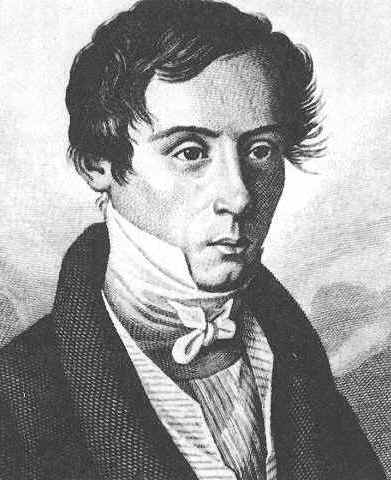
\includegraphics{numeric/figures/a_fresnel}
  \caption{Augustin-Jean Fresnel (1788-1827)}
\end{marginfigure}

Finally, we want to point out the similarity in structure between Eq.~\ref{Eq:MM 5a} and \ref{Eq:MM 5b} and the well--known Fresnel equations to calculate reflection and transmission for normal incidence of a plane wave upon the interface between two semi--infinite media:

\begin{eqnarray}
T & = & \frac{2n_{1}}{n_{1}+n_{2}}\label{Eq:T normal} \\
R & = & \frac{n_{1}-n_{2}}{n_{1}+n_{2}}\label{Eq:R normal} 
\end{eqnarray}

In fact, Eq.~\ref{Eq:T normal} and \ref{Eq:R normal} can also be derived from the more general treatment presented here. For homogeneous layers, where the refractive index does not vary in the transverse direction, it turns out that the overlap matrices are diagonal, meaning that there is no cross--coupling between the different modes. Further evaluation of the formula's reveals that the Fresnel equations are indeed recovered.

Obviously, a realistic structure will consist of more than one interface, but that problem is outside the scope of this text.


\begin{exer}
% difficulty: hard
Derive the matrix form for the eigenmode expansion equations for the reflection and the transmission matrix at an interface, in case the basis functions are not orthogonal.

\begin{sol}
$$ \begin{bmatrix} \mathbf{O}^{T}_{II,I} & -\mathbf{O}^{T}_{I,I} \\ \mathbf{O}_{I,II} & \mathbf{O}_{I,I} \end{bmatrix} \begin{bmatrix} \mathbf{T}_{I,II} \\ \mathbf{R}_{I,II} \end{bmatrix} =  \begin{bmatrix} \mathbf{O}^{T}_{I,I} \\ \mathbf{O}_{I,I} \end{bmatrix} $$
\end{sol}

\end{exer}


\pagebreak


\sectionugent{Method of weighted residuals}

To conclude this chapter, we will present the method of weighted residuals, a very general scheme for converting linear differential and integral equations into a form suitable for numerical solution by standard matrix methods.

We start from a problem of the type

\begin{equation}
L u = v \label{eq-operator}
\end{equation}

where $v$ represents some known excitation and $u$ is the unknown and wanted field. $L$ is a linear operator involving differentiation, integration or both.

\begin{cue}
Cast the Helmholtz equation in this form.  
\end{cue}

For the Helmholtz equation, $v=0$ and $L=\nabla^2 + k^2$. 

Suppose we approximate the unknown $u$ by

\begin{equation}
\tilde{u}(x) = \sum_{i=1}^N u_i b_i(x) \label{eq-expansion}
\end{equation} 

where $b_i(x)$ are a complete set of known basis functions. The general problem is now to choose the coefficients $u_i$ to approximate as well as possible the unknown solution $u$ to Eq.~\ref{eq-operator} with a \emph{finite} number $N$ of basis functions.

\begin{cue}
How would you quantify 'as well as possible'? Is the method you propose useful in practice?  
\end{cue}

Your first hunch could be to try and minimise the difference between the exact solution $u$ and its approximation $\tilde{u}$. However, this will get you nowhere in practice: you don't know the exact solution, so you cannot evaluate the difference.

\begin{cue}
What happens if you apply $L$ to the difference between $u$ and $\tilde{u}$? 
\end{cue}

Doing this, leads to the definition of the \textbf{error residual}:

\begin{equation}
R(x) = L\tilde{u} - v = L \sum_{i=1}^N u_i b_i(x) - v(x)
\end{equation} 

which is clearly zero if and only if we have an exact solution to Eq.~\ref{eq-operator}. Moreover, apart from the coefficients $u_i$, all the other quantities can be calculated. Now we have a realistic objective: trying to make the residual as small as possible.

\begin{cue}
Think about how you would quantify and minimise the size of this residual. 
\end{cue}

There are many approaches you could take here, e.g. asking that the energy of the residual is minimised, or imposing that the residual vanishes at a set of predefined points.

Here however, we will introduce a more general approach, of which the examples listed above are special cases.

\noindent\marginnote{Don't confuse the weight functions $w_i$ with the weight function you could choose to define your scalar product, e.g. $r$ in the scalar product of Bessel functions. These are completely independent choices.}To proceed, we choose another set of functions, the so--called \textbf{test} or \textbf{weight} functions $w_i$. We also introduce an inner product (scalar product) formally written as $\langle f(x),g(x) \rangle$. The definition of the inner product is in a sense arbitrary and often follows from the specifics of the problem considered.

Rather than asking the impossible that $R(x)=0$ for all $x$, we insist that $R(x)$ be orthogonal to each of the weight functions under the scalar product considered.

\begin{cue}
Impose this condition and put it in matrix form.  
\end{cue}

This results in the following $N$ equations for $N$ unknowns:

\begin{equation}
\left\langle \left\{ L \sum_{i=1}^N u_i b_i(x) - v(x)  \right\}, w_j(x) \right\rangle = 0 \hspace{0.5cm} j=1,2\cdots,N \label{eq-weighted-res}
\end{equation}

In the above equation, $b_i(x)$, $v(x)$ and $w_j(x)$ are known functions of $x$. $L$ is the known operator and $u_i$ are the unknown and wanted scalars which when put into Eq.~\ref{eq-expansion} give our approximate solution.

Because of the linearity of Eq.~\ref{eq-weighted-res}, it can be put into a compact matrix form:

\begin{equation}
{\mathbf L} \cdot {\mathbf u} = {\mathbf v}
\end{equation} 

Here, $\mathbf u$ denotes the unknown column vector containing $u_1, u_2, \hdots, u_N$. $\mathbf v$ denotes the known column vector with elements $\left\langle v(x), w_j(x) \right\rangle$. Finally ${\mathbf L}$ is a known $N \times N$ matrix with $(i,j)$-th element $\left\langle L b_i(x), w_j(x) \right\rangle$.

So, our equation $Lu=v$ has been \emph{projected} by approximation into the matrix equation ${\mathbf L} \cdot {\mathbf u} = {\mathbf v}$, which can be solved with standard numerical routines.

Apart from the the weighted residuals method, the above procedure is also called the \textbf{method of moments} or the \textbf{generalised Galerkin method}.

\subsection{Choice of basis and test functions}

\begin{marginfigure}[-.0cm]
  % credits: Wikipedia
  % url:  https://en.wikipedia.org/wiki/Boris_Galerkin
  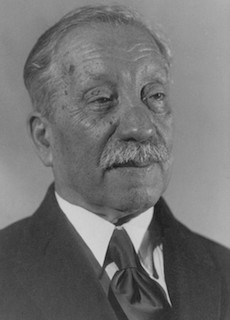
\includegraphics{numeric/figures/b_galerkin}
  \caption{Boris Grigoryevich Galerkin (1871-1945)}
\end{marginfigure}

Starting from the general procedure outlined above, different numerical methods can be derived that are catalogued according to their choice of basis and test functions.

If basis and test functions are chosen equal, i.e. $b_i(x) = w_i(x)$, the the method is called the (non--generalised) \textbf{Galerkin method}. Often this leads to a formulation which can be cast in a variational form, having the advantages already outlined previously.

Another choice is

\begin{equation}
w_j(x) = \delta(x-x_j)
\end{equation} 

\begin{cue}
What will be the effect of choosing the test functions that way?  
\end{cue}

This corresponds to demanding the the error residual vanishes exactly at the points $x_j$ when the scalar product is defined as the integral of the product:

\begin{equation}
\left\langle R(x), w_j(x) \right\rangle = \int R(x) \delta(x-x_j) dx = R(x_j) = 0
\end{equation} 

This is called the \textbf{point matching} or \textbf{collocation method}.

Another interesting choice is explored in the following exercise:

\begin{exer}
% difficulty: normal
% ugent
% youtube: ZdapTpUOIrE  
Assuming a commutative scalar product, show that the choice 

$$w_i(x) = L b_i(x)$$

leads to the minimisation of the norm of the error residual 

$$\left\langle R(x), R(x) \right\rangle$$ 

Because of this property, this choice is called the \textbf{least-squares residual} method.
\end{exer}

\pagebreak

\begin{exer}
% difficulty: normal   
In the least-squares residual method, what is the geometrical interpretation of imposing that 

$$\left\langle R(x), w_j(x) \right\rangle$$ 

for all values of $j$?
\end{exer}



\begin{exer}
% difficulty: normal  
Construct an example where the Galerkin method and the least-squares residual method are identical.
\end{exer}



\section*{Review questions}

\begin{itemize}
\item What are the advantages and disadvantages of the different numerical methods for photonics? In what circumstances would you use them?
\item What is the difference between forward, backward and central difference approximations to the derivative?
\item How does the finite-element method distinguish itself from other methods?
\item What is the Rayleigh-Ritz method?
\item What is a functional?
\item What is a variational problem? Stationarity? First variation?
\item What is the Euler-Lagrange equation of a variational problem?
\item For what problems is eigenmode expansion best used?
\item What are some common choices for test functions in the method of weighted residuals?  
\end{itemize}

%%% Local Variables:
%%% mode: latex
%%% TeX-master: "../main"
%%% End:
